\documentclass{article}
\usepackage[utf8]{inputenc}
\usepackage{amsmath}
\usepackage{tikz}
\usepackage{hyperref}
\usepackage{mathdots}
\usepackage{yhmath}
\usepackage{cancel}
\usepackage{color}
\usepackage{siunitx}
\usepackage{array}
\usepackage{multirow}
\usepackage{amssymb}
\usepackage{tabularx}
\usepackage{booktabs}
\usepackage{graphicx}
\usepackage[margin=1in]{geometry}
\usepackage{imakeidx}
\usepackage{titlesec}
\usepackage{pdfpages}
\usepackage{listings}
\usepackage{systeme}
\usepackage[normalem]{ulem}
\useunder{\uline}{\ul}{}

\pagestyle{headings}

\definecolor{keywords}{RGB}{255,0,90}
\definecolor{comments}{RGB}{0,0,113}
\definecolor{red}{RGB}{160,0,0}
\definecolor{green}{RGB}{0,150,0}

\lstset{language=c++, 
        basicstyle=\ttfamily\small, 
        keywordstyle=\color{keywords},
        commentstyle=\color{comments},
        stringstyle=\color{red},
        showstringspaces=false,
        identifierstyle=\color{green},
        keywords=[2]{pow},
        keywordstyle=[2]{\color{orange}},
        keywords=[3]{REFERENCES},
        keywords=[4]{string},
        keywords=[5]{mapping},
        keywords=[6]{address},
        keywords=[7]{function},
        keywords=[8]{memory},
        keywordstyle=[3]{\color{keywords}},
}


\pagenumbering{Roman}

\title{Cloudest Paper}
\author{Filippo Scaramuzza, Luca Pastori}
\date{A.A. 2020/2021}

\begin{document} 
\begin{titlepage}
	\centering
	
\includegraphics[width=0.15\textwidth]{images/unipr_centrato_2righe_pos_rgb.jpg}\par\vspace{1cm}
	{\scshape\LARGE Università degli Studi di Parma \par}
	\vspace{1cm}
	{\scshape\Large Ingegneria Informatica Elettronica e delle Telecomunicazioni\\
	Ingegneria dei Sistemi Informativi\\\par}
	\vspace{0.5cm}
	{\scshape\Large Tecnologie Internet\par}
	\vspace{1.5cm}
	{\huge\bfseries Cloudest\\
	Cloud storage decentralizzato basato sulla blockchain Ethereum e IPFS \par}
	\vspace{2cm}
	{\Large\itshape Filippo Scaramuzza\\Luca Pastori\par}
	\vfill

	{\large A.A. 2020/2021 \par}
\end{titlepage}


\newpage

\tableofcontents
\newpage
\pagenumbering{arabic}
\setcounter{page}{1}

\section{Introduzione}

\subsection{Il problema}
Secondo un articolo di SeedScientific \cite{seed_scientific_article}, ogni giorno vengono prodotti 2,5 quintilioni di byte di dati. Va notato che sul totale dei dati nel mondo, oltre il 90\% dei dati è stato prodotto negli ultimi 4 anni. La maggior parte dei dati attualmente disponibile attraverso Internet è però "centralizzata", ovvero archiviata da un numero molto ristretto di aziende tecnologiche che hanno l'esperienza e il capitale per costruire enormi data center in grado di gestire queste enormi quantità di dati. Il problema fondamentale di questo approccio è proprio la centralità dei dati. Questi ultimi infatti sono alla mercé di malintenzionati che possono accedere, modificare o addirittura cancellare i dati caricati nei data center. Quando si parla di aziende molto grandi questo è un rischio molto basso, ma un altro grande problema è dietro l'angolo. Ciò che è più importante per un consumatore è la sua privacy, molto spesso messa a repentaglio da agenzie terze che utilizzano i dati caricati per fini di marketing e pubblicità, spesso all'insaputa dei consumatori. Inoltre, il costo sostenuto per l'archiviazione dei dati in server centralizzati è molto alto e di grande impatto sull'ambiente e molte volte gli utenti finali devono pagare per un piano di archivazione anche se utilizzano solo una minima parte dello spazio che hanno effettivamente comprato. Un ulteriore problema è la scalabilità del sistema: è infatti difficile scalare un sistema di archiviazione centralizzato per soddisfare la crescente domanda.

\subsection{La possibile soluzione}
La piattaforma che questa relazione vuole descrivere, Cloudest, tenta di risolvere i numerosi problemi tecnici, etici ed economici dell'attuale sistema di archiviazione centralizzato. 

La blockchain è di fatto un sistema di cloud storage decentralizzato che garantisce la sicurezza dei dati. Qualsiasi nodo di elaborazione connesso a Internet può unirsi e formare una rete di peer, massimizzando così l'utilizzo delle risorse. Ogni nodo della rete memorizza una copia della blockchain rendendola così immutabile. In Cloudest l'utente può caricare un file sulla piattaforma che a sua volta invia la risorsa alla rete P2P IPFS (\textit{InterPlanetary File System}). Come si vedrà nel seguito, IPFS utilizza un sistema di \textit{hash} per recuperare i file distribuiti nella rete, Cloudest si occupa di salvare questi hash e renderli disponibili salvandoli con tutte le informazioni necessarie sulla blockchain.

\newpage
\section{L'architettura di Sistema}
\subsection{Struttura e schema generale}
Cloudest, raggiungibile al link \href{https://cloudest.cloud}{https://cloudest.cloud} è un'\textit{applicazione decentralizzata}, struttura anche conosciuta come \textit{DApp}, appunto \textit{Decentralized Application}. La struttura può essere rappresentata come mostrato in Figura \ref{fig:dapp_architecture.jpg}.
\\

\begin{figure}[!ht]
  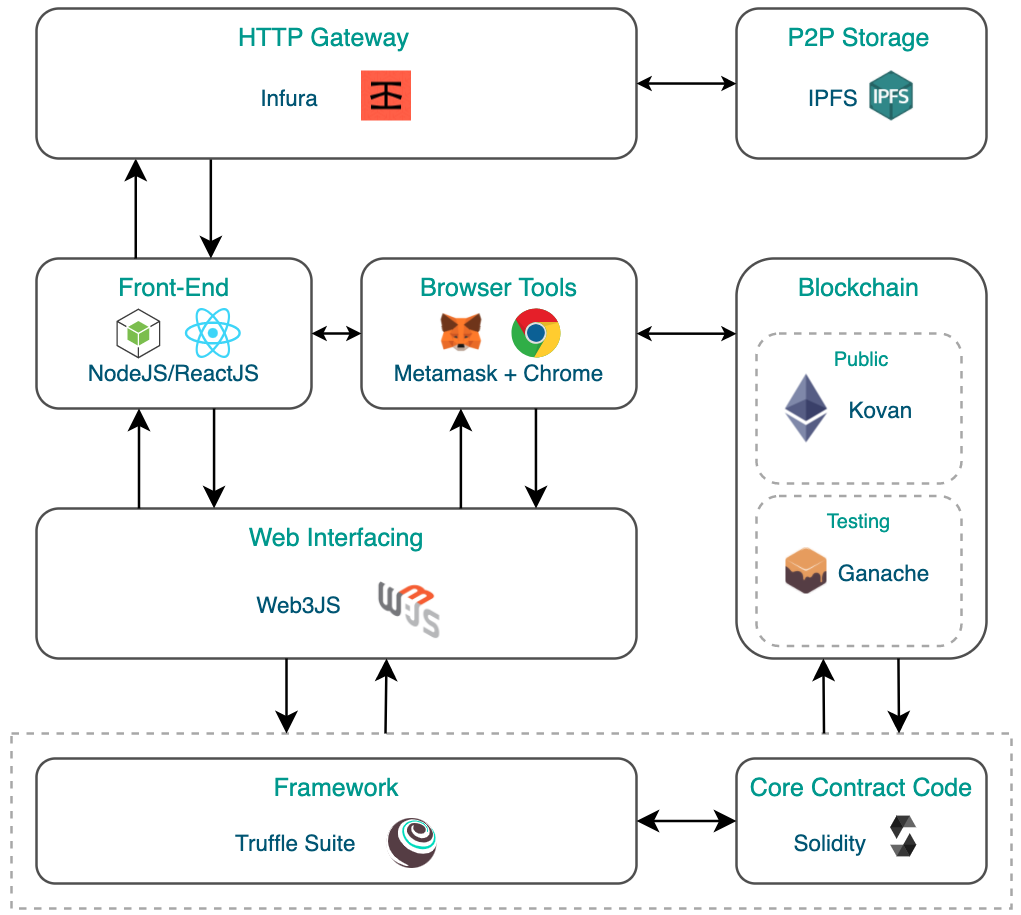
\includegraphics[width=16cm]{images/dapp_architecture.png}
  \centering
  \caption{Architettura di Cloudest}
  \label{fig:dapp_architecture.jpg}
\end{figure}

Di seguito viene fatta una breve descrizione delle componenti principali.

\subsection{Framework: Truffle Suite}
\textit{Truffle} \cite{truffle_suite} è un framework di test e una pipeline di risorse per la blockchain che utilizza la \textit{Macchina Virtuale Ethereum} (EVM), con l'obiettivo di \textit{semplificare} la vita agli sviluppatori. Fornisce infatti una serie di strumenti volti alla migrazione di contratti sulle reti private e pubbliche ed una serie di strumenti per l'integrazione con le Web App, in particolare interfacciandosi con la libreria Web3JS.

\subsection{Core Contract Code: Solidity}
\textit{Solidity} \cite{solidity} è un linguaggio ad alto livello orientato agli oggetti utilizzato per l'implementazione di \textit{smart contracts}. Nello specifico caso di Cloudest, viene utilizzato un solo contratto (si veda nel seguito) che si occupa di organizzare tramite particolari strutture i dettagli dei file associandoli ai singoli utenti.

\subsection{Web Interfacing: Web3JS}
Web3JS \cite{web3js} è una libreria scritta interamente in Javascript che permette l'interazione, tramite opportuni strumenti, ad esempio Metamask (si veda nel seguito), con la blockchain, nel caso di Cloudest tramite HTTP.
Infatti una volta che viene eseguito il comando \texttt{truffle compile} (comando specifico per la compilazione di contratti della suite di Truffle), viene creato un file \texttt{json} relativo al contratto che Web3JS interpreta, richiamando ad esempio specifiche funzioni del contratto dal codice Javascript.

\subsection{Front-End e Browser Tools}
\subsubsection{NodeJS/ReactJS}
Cloudest utilizza come \textit{client} un'applicazione Javascript che utilizza NodeJS \cite{nodejs}, in particolare ReactJS \cite{reactjs} per gestire la parte grafica. Lo scopo di React è quello di visualizzare i dati recuperati dalla blockchain e da IPFS mostrandoli all'utente e fornisce gli strumenti (bottoni, textbox, ecc...) per l'interazione con l'applicazione e IPFS nonché con la blockchain.

\subsubsection{Metamask + Chrome}
Lo sviluppo di Cloudest è stato orientato ad un suo utilizzo su Chrome, scelta fatta considerando soprattutto l'utilizzo dell'estensione \textit{Metamask} \cite{metamask}, ben integrata con Chrome. Metamask è di fatto un wallet per Ethereum, che si integra alla perfezione con le applicazioni sviluppate ad esempio in javascript, e soprattutto con Web3JS. Infatti fornisce un modo semplice per effettuare le transazioni necessarie per l'utilizzo dei contratti e permette di effettuare uno \textit{switch} rapido tra reti Ethereum differenti.

\subsection{Blockchain}
\subsubsection{Testing: Ganache}
\textit{Ganache} \cite{ganache} è una blockchain personale per lo sviluppo rapido di applicazioni distribuite Ethereum e Corda. È possibile utilizzare Ganache in tutto il ciclo di sviluppo, consentendo di sviluppare, distribuire e testare le DApps in un ambiente sicuro e deterministico.
\subsubsection{Public: Kovan}
\textit{Kovan} \cite{kovan} è una blockchain \textit{Proof of Authority} (PoA) accessibile al pubblico di Ethereum;Questa nuova testnet utilizzerà Parity (un client Ethereum sviluppato da Parity Technologies, FKA Ethcore) per fornire un ambiente testnet stabile e sicuro per gli sviluppatori Ethereum. Si è deciso di utilizzare Kovan come testnet e non reti più conosciute come ropsten data la sua stabilità e velocità nell'elaborare nuove transazioni.

\subsection{HTTP Gateway: Infura}
\textit{Infura} \cite{infura} è un framework che fornisce diversi servizi sia per l'interazione con la blockchain di Ethereum (ad esempio per il \textit{deploy} dei contratti su reti pubbliche, fungendo da \textit{HTTP Provider}) o per l'interazione con IPFS (fungendo da \textit{Gateway}). Nel caso di cloudest Infura è stato utilizzato sia per interagire con IPFS che per effettuare il deploy del contratto sulla rete \textit{Kovan}.

\subsection{P2P Storage: IPFS}
\textit{IPFS} \cite{ipfs}, \textit{Interplanetary File System} è un protocollo hypermedia distribuito peer-to-peer open source che mira a funzionare come un file system per tutti i dispositivi di elaborazione connessi. Il suo funzionamento consiste nel suddividere i file, ai quali viene assegnato un identificatore univoco un hash crittografico, in blocchi e distribuiti ai nodi della rete. I duplicati vengono rimossi attraverso la rete e la cronologia delle versioni viene tracciata per ogni file. Ciò porta a contenuti permanentemente disponibili, inoltre, l’autenticità del contenuto è garantita attraverso questo meccanismo e, quando un dispositivo cerca i file, si chiede essenzialmente alla rete di trovare nodi che memorizzano il contenuto dietro l’hash di identificazione univoco associato a quel contenuto.

\newpage
\section{Lo sviluppo di Cloudest}
In questa sezione verranno mostrati e citati gli strumenti e le tecnologie utilizzate per lo sviluppo e per la gestione del progetto Cloudest.

\subsection{Organizzazione e Time Management}
Lo sviluppo di Cloudest è stato suddiviso in 3 grandi \textit{milestone}. 
\subsubsection{Milestone 1: Faucet}
Nella prima lo sviluppo è stato incentrato su una semplice applicazione che fungeva da \textit{Faucet} (una sorta di "banca" per ethereum. Un utente può contattare il Faucet così da richiedere una somma in Ether. E' uno strumento comune, naturalmente, solo nelle testnet). Da questa applicazione in particolare si può anche contribuire a fornire fondi al Faucet. Questa prima milestone è servita per prendere dimestichezza con l'interazione con Metamask e con i contratti sulla blockchain. In Figura \ref{fig:faucet} uno screenshot dell'applicazione.
\begin{figure}[!ht]
  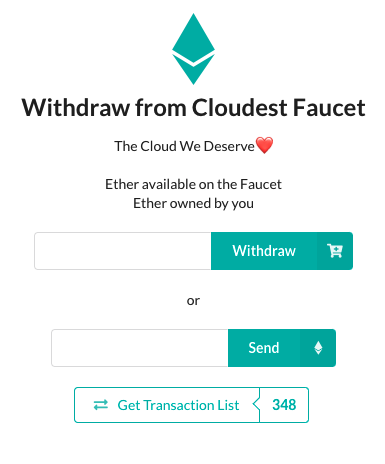
\includegraphics[width=8cm]{images/faucet.png}
  \centering
  \caption{Cloudest Faucet User Interface}
  \label{fig:faucet}
\end{figure}

\subsubsection{Milestone 2: prima integrazione con IPFS}
La seconda milestone è servita a prendere dimestichezza con il sistema \textit{Infura + IPFS}. In questa semplice applicazione è stato testato l'upload e il download di un singolo file dalla rete IPFS. Uno screenshot dell'applicazione è in Figura \ref{fig:ipfs}.
\begin{figure}[!ht]
  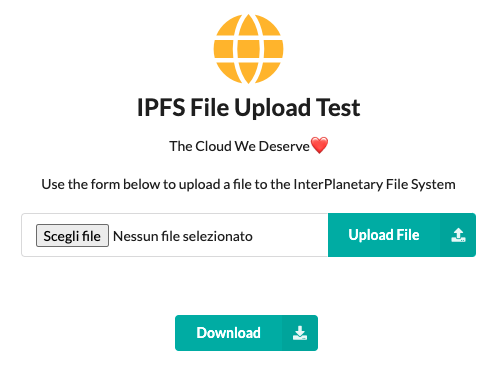
\includegraphics[width=10cm]{images/ipfs.png}
  \centering
  \caption{Test di upload/download IPFS}
  \label{fig:ipfs}
\end{figure}

\subsubsection{Milestone 3: Integrazione e sviluppo della Piattaforma}
La terza e ultima milestone, nonché la più corposa, è stata volta allo sviluppo della piattaforma vera e propria, come integrazione delle due milestone precedenti e delle varie funzionalità e scrittura del contratto.

\subsection{Time/Tasks Management e Sviluppo}
\subsubsection{Time/Tasks Management}
Per la gestione dei tasks, del tempo, delle scadenze e in generale per l'organizzazione di un progetto di per se piuttosto complesso è stata utilizzata la piattaforma \textit{Microsoft Planner} \cite{microsoft_planner}, di cui è riportato uno screenshot in Figura \ref{fig:planner}.
\begin{figure}[!ht]
  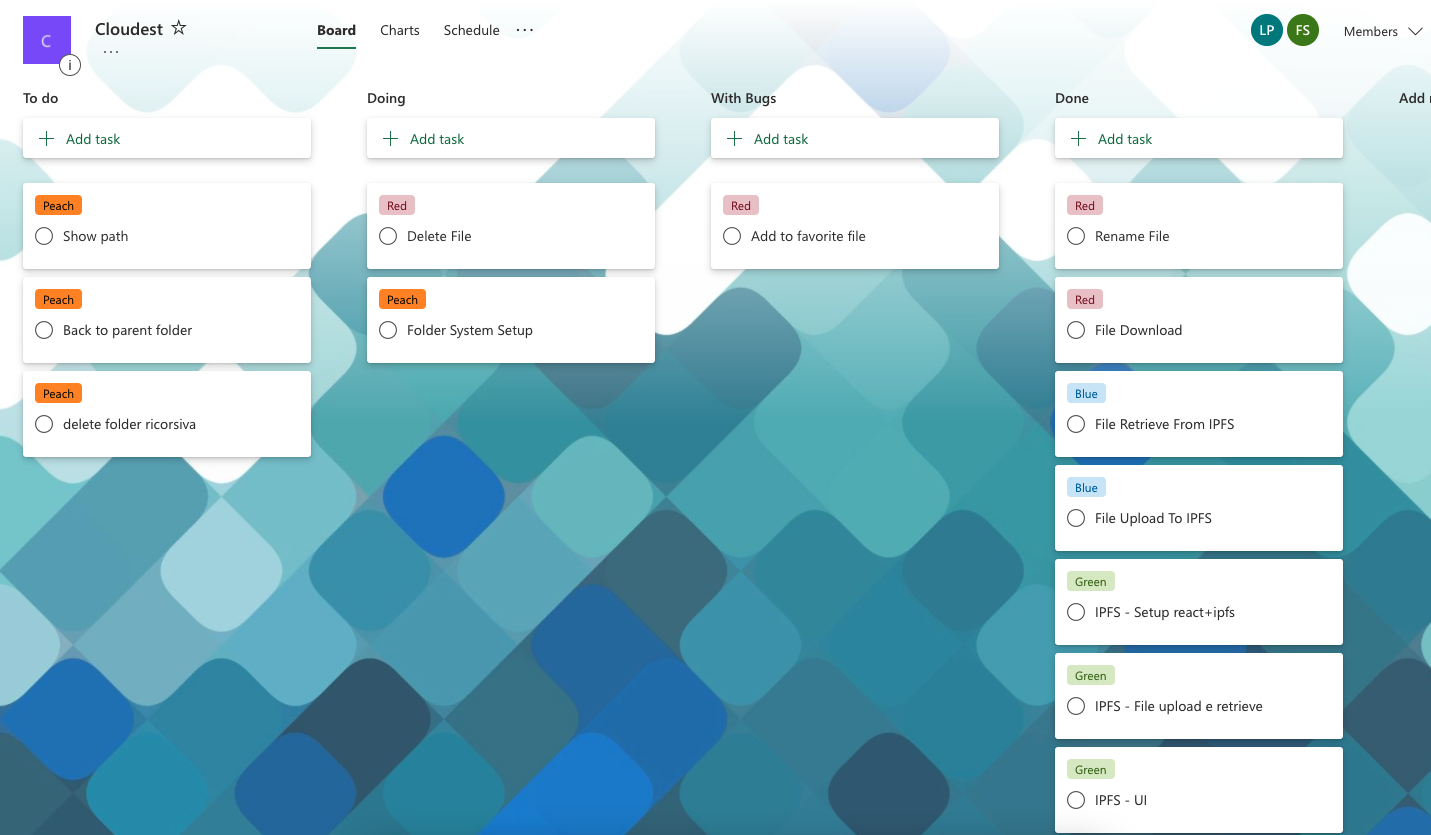
\includegraphics[width=16cm]{images/planner.png}
  \centering
  \caption{Microsoft Planner}
  \label{fig:planner}
\end{figure}

\subsubsection{Sviluppo}
Per conservare in modalità sicura il codice scritto si è utilizzato Github un'applicazione utile per store e versioning del codice.
Per lo sviluppo della piattaforma è stato utilizzato interamente Visual Studio Code \cite{vs_code}, scelto per la sua semplicità e comodità d'uso, nonché per le sue funzionalità. Infatti per renderlo idoneo all'utilizzo sono state aggiunte alcune estensioni come ad esempio \textit{Live Shere} utile per lo sviluppo simultaneo di codice in tempo reale. Con questa estensione è stato anche possibile condividere il server di sviluppo (\texttt{localhost}) su tutti i dispositivi connessi alla sessione di Live Share, così da poter operare e visualizzare contemporaneamente il codice e il suo effettivo funzionamento, come se fosse un solo computer.

Grazie a questi strumenti è stato possibile sviluppare l'intera piattaforma interamente a distanza.

\newpage
\section{Il funzionamento e l'utilizzo di Cloudest}

Per ogni sezione viene mostrato il funzionamento della piattaforma dal lato dell'utente finale (Foreground) e dal lato della piattaforma, con i dettagli tecnici sul funzionamento (Background).

\subsection{Avvio e "login"}
\subsubsection{Foreground}
Quando l'utente si reca su \href{https://cloudest.cloud}{https://cloudest.cloud} questa è la schermata che gli si presenta (Figura \ref{fig:login}).
\begin{figure}[!ht]
  \includegraphics[width=14cm]{images/login.png}
  \centering
  \caption{Avvio e login}
  \label{fig:login}
\end{figure}
Se tutto funziona correttamente, Metamask propone all'utente di fare il login e sbloccare il portafoglio, così da permettere all'applicazione di accedere a quest'ultimo. Se di nuovo tutto funziona correttamente all'utente viene mostrata la pagina dell'applicazione vera e propria, di cui uno screenshot è mostrato in Figura \ref{fig:home}.
\begin{figure}[!ht]
  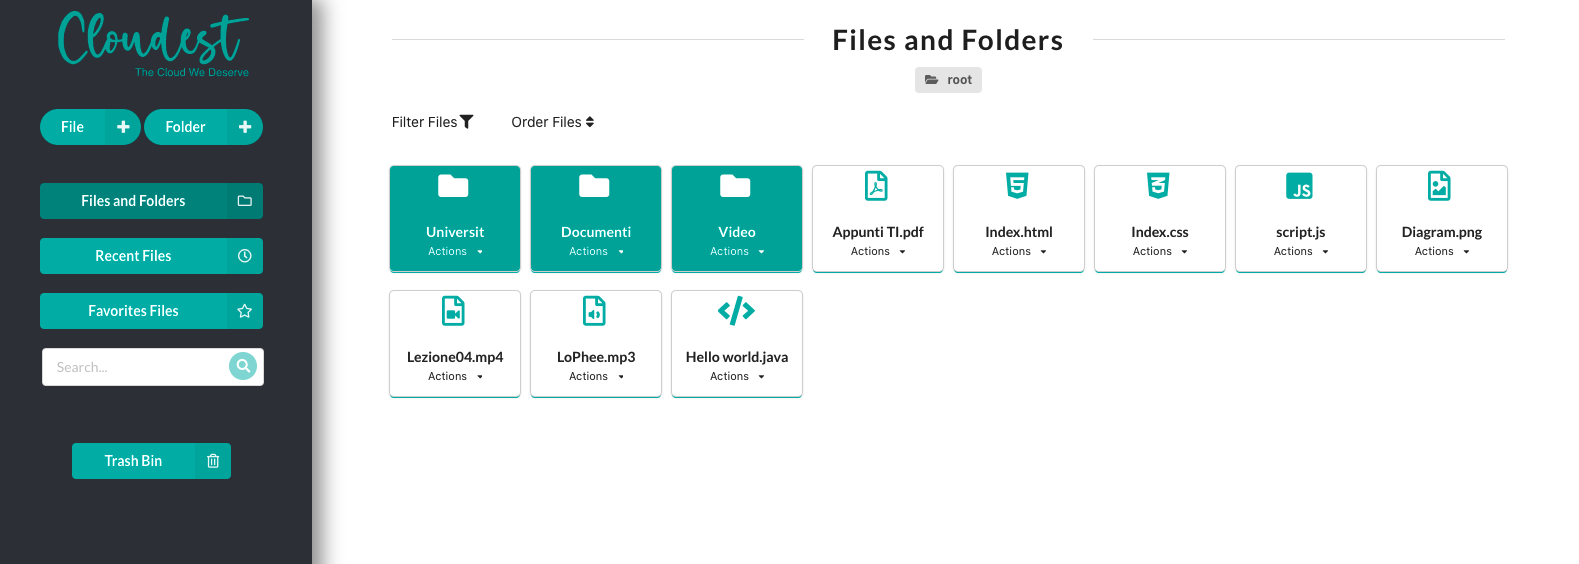
\includegraphics[width=16cm]{images/home.png}
  \centering
  \caption{Home di Cloudest}
  \label{fig:home}
\end{figure}

\subsubsection{Background}
Ciò che accade "dietro le quinte" è ciò che consente a Metamask e all'applicazione React di comunicare. Tramite una particolare funzione (\texttt{getWeb3()}), viene recuperato l'oggetto Javascript \texttt{web3} dall'oggetto \texttt{window}. Questo oggetto è fornito direttamente da Metamask e permette di comunicare con la libreria Web3JS.

\subsection{Upload di un file/cartella}
\subsubsection{Foreground}
L'utente cliccando sul pulsante "File +" può caricare un file dal popup che gli viene mostrato. Una volta confermato il caricamento su IPFS viene mostrato all'utente il popup di Metamask che chiede la conferma della transazione. In Figura \ref{fig:fileupload} si può vedere uno screenshot della funzionalità di upload.

\begin{figure}[!ht]
  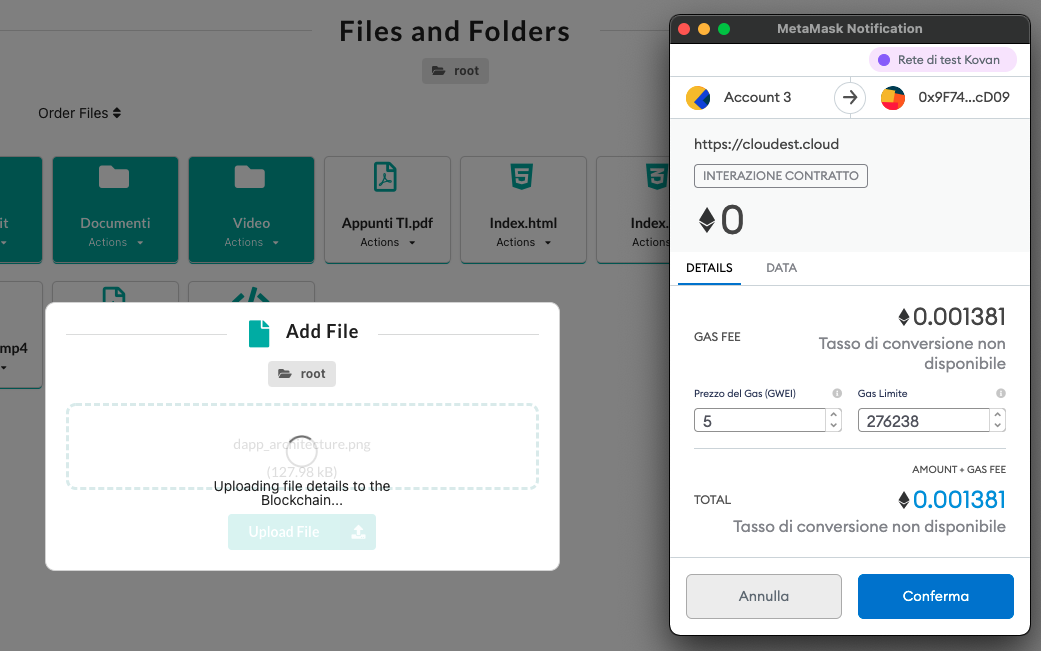
\includegraphics[width=14cm]{images/fileupload.png}
  \centering
  \caption{Home di Cloudest}
  \label{fig:fileupload}
\end{figure}

La procedura per la creazione di una cartella è pressoché identica a quella dell'upload di un file.

\subsubsection{Background}
Per quanto riguarda l'upload dei File, vengono richiamate principalmente due funzioni. Con la prima il file viene caricato sulla rete IPFS. Questa funzione restituisce poi l'hash identificativo del file, che viene caricato insieme a tutte le informazioni sulla blockchain dalla seconda funzione richiamata. 

Le cartelle vengono trattate dallo smart contract esattamente come un file, il cui tipo è però \texttt{folder}. Il sistema di cartelle e sottocartelle è stato implementato tramite l'aggiunta di un attributo \texttt{parentFolder} ad ogni file e ad ogni cartella, in modo tale che sia possibile ricostruire \textit{on demand} la struttura ad albero del filesystem, permettendo anche
la cancellazione \textit{ricorsiva} dei file e delle sottocartelle che li contengono.

 Il file, o meglio, il suo buffer, viene cifrato prima di essere caricato sulla rete IPFS tramite l'algoritmo \textit{AES-256} utilizzando come chiave di cifratura l'hash di 32 byte dell'indirizzo del portafoglio dell'utente ottenuto tramite l'algoritmo di hashing \textit{keccak256}.

\subsection{Download, Rename File e Add To Favorite}
\subsubsection{Foreground}
L'utente premendo in "action", link visibile in ogni file e cartella, ha accesso alle funzioni quali download dell'elemento, rinominarlo o l'aggiunta dei favoriti. In figura \ref{fig:renameFavorite} si può vedere uno screenshot delle funzionalità di download, rename e add to file.
\begin{figure}[!ht]
  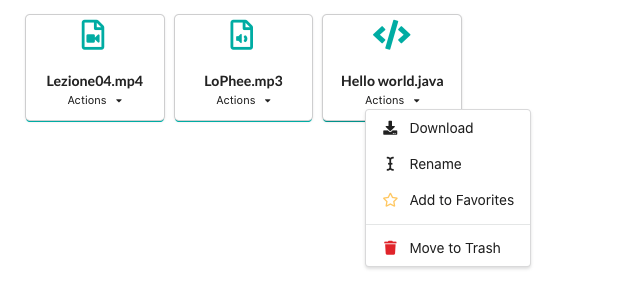
\includegraphics[width=14cm]{images/renameFavorite.png}
  \centering
  \caption{Download, Rename File e Add To Favorite}
  \label{fig:renameFavorite}
\end{figure}

\subsubsection{Background}
Quando l'utente preme su "Download" viene recuperato il buffer del file dalla rete IPFS tramite l'hash del suddetto file per essere decifrato. A questo punto il file viene scaricato tramite la funzione \texttt{fileDownload()} con tutte le informazioni relative (quali nome ed estensione) recuperate dal contratto. Sia nel caso di "Rename" che nel caso di "Add/Remove to Favorites", c'è il richiamo ad una specifica funzione del contratto che si occupa di modificare gli attributi del file secondo l'evenienza. Di seguito verrà approfondito il contratto e la sua struttura.

\subsection{Move to Trash e Delete Definitively}
\subsubsection{Foreground}
Quando si desidera eliminare un file per prima cosa l'utente dovrà spostarlo nel cestino. All'interno di esso si potrà scegliere se eliminare definitamente il file/cartella oppure recuperarlo e riportarlo nella posizione originaria. In Figura \ref{fig:moveTrash} si può vedere uno screenshot delle funzionalità di delete.

\begin{figure}[!ht]
  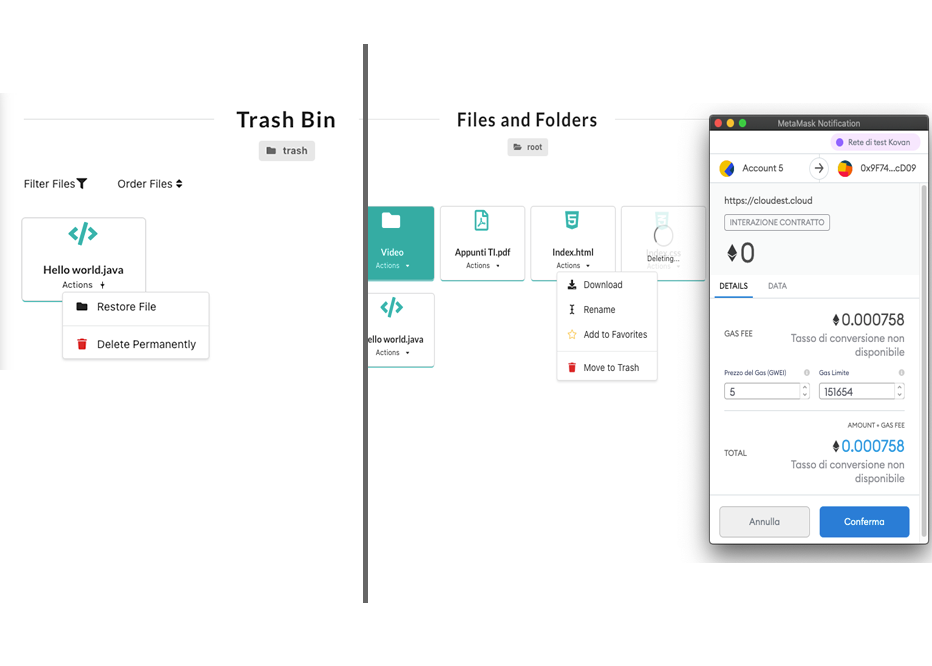
\includegraphics[width=14cm]{images/moveTrash.png}
  \centering
  \caption{Move to Trash e Delete Definitively}
  \label{fig:moveTrash}
\end{figure}

\subsubsection{Background}
Come accennato sopra il sistema di foldering è basato sul concetto di \textit{parent folder}, così da poter effettuare, se necessaria una cancellazione ricorsiva. C'è infatti un particolare metodo nel contratto che verrà approfondito in seguito, in cui in modo ricorsivo vengono spostati i file nel cestino oppure eliminati definitivamente. Va notato che se si sposta una cartella nel cestino ogni file e cartella al suo interno verranno spostati nel cestino, per essere eventualmente spostati nella cartella root se recuperati dal cestino. Questo implica quindi che la struttura di cartelle e sottocartelle viene mantenuta solo se ad essere spostata nel cestino è una intera cartella.

\subsection{File Preferiti, File Recenti, Ricerca e Filtri}
\subsubsection{Foreground}
L'utente può, tramite i pulsanti nella barra di navigazione laterale, spostarsi tra la pagina che contiene tutte le cartelle, sottocartelle e file cliccando su "Files and Folders", oppure spostarsi nelle pagine "Favorites Files", che mostra i file marcati come \textit{favorite}, e "Recent Files". In questa pagina è possibile visionare tramite opportuni filtri i file caricati nell'ultima ora, nella giornata corrente, nell'ultima settimana o nell'ultimo mese.

Vari filtri sono stati implementati anche nella pagina "Files and Folders", dando così all'utente la possibilità di visualizzare solo alcuni tipi di file oppure ordinarli secondo data o nome (crescenti o decrescenti).

E' stata inoltre implementata la funzione di ricerca (anch'essa accessibile dalla barra laterale), che permette di ricercare qualsiasi tipo di file dal suo nome, in tutte le cartelle e sottocartelle.

\subsubsection{Background}
Tutte le funzionalità sopra esposte sono state realizzate tramite le funzioni di React. In particolar modo è stato utilizzato durante tutto lo sviluppo il concetto di \textit{state}, caratteristico delle compoenenti di React, che permette di memorizzare dati (e.g. la cartella corrente in cui si trova l'utente), aggiornarli e modificarli, innescando così determinate azioni. L'utilizzo di questi meccanismi ha fatto sì che sia stato possibile realizzare una cosiddetta \textit{single-page application}, in \textit{real-time} (i.e. senza la necessità di aggiornare la pagina per ristabilire la connessione con Node, mantenendo infatti una connessione costante).

\newpage

\section{Il contratto FileDetailsManager.sol}
\textit{FileDetailsManager} è il nucleo di tutta la piattaforma. Come accennato nelle sezioni precedenti, \textit{FileDetailsManager} è uno \textit{smart contract} il cui scopo fondamentale è quello di gestire, memorizzandoli e modificandoli, i dati dei singoli utilizzatori di Cloudest. Qesti \textit{dati}, non sono i dati personali (si ricorda che lo scopo della piattaforma è anche quello di mantenere la password), bensì i dettagli dei file che gli utenti caricano nel "cloud" tramite Cloudest.
\subsection{Strutture dati}
\subsubsection{Struttura "FileDetails"}
I dettagli di ogni singolo file sono salvati in una particolare struttura dati (una \texttt{struct}), così formata:

\begin{lstlisting}
    struct FileDetails {
        string uniqueId; //unique id of the folder or the file's IPFS fileHash
        string name; // folder's name or file's name
        string transactionDate; // The date in which file's info was stored
        string fileType; // "folder" if folder otherwise the extension of the file
        string parentFolderId; // parent folder id (both for files and folders)
        bool isFavorite; // true if favorite, false otherwise
        bool isTrash; // true if currently in the trash, false otherwise
    }
\end{lstlisting}

Come si può notare ad ogni "file" è associato il suo hash relativo ad IPFS, mentre ad ogni cartella (che si ipotizza possano avere nomi uguali), è associato un indirizzo univoco. Questo viene calcolato tramite un contatore che viene incrementato ogni volta che una cartella viene creata.

\subsubsection{Mapping wallet $\rightarrow$ fileDetails}
Come accennato sopra, ad ogni utente, o per meglio dire ad ogni \textit{wallet} che interagisce con il contratto aggiungendo file, è assegnato un array contenente tutti i dettagli di tutti i file aggiunti. Per fare questo è stata utilizzata una struttura dati chiamata \texttt{mapping}, come segue:

\begin{lstlisting}
    mapping(address => FileDetails[]) filesList;
\end{lstlisting}

\subsection{Metodi}

\subsubsection{AddFile}

\begin{lstlisting}
    function addFile(string memory uniqueId, 
                 string memory name, 
                 string memory fileType, 
                 string memory date, 
                 string memory parentFolderId) 
\end{lstlisting}

Questo metodo serve ad aggiungere un file all'array dei file di uno specifico \textit{wallet}, con i dati specificati nei parametri.

\subsubsection{AddFolder}

\begin{lstlisting}
    function addFolder(string memory name, 
                       string memory date, 
                       string memory parentFolderId) 
\end{lstlisting}

    Questo metodo serve ad aggiungere una cartella all'array di uno specifico \textit{wallet}, con i dati specificati nei parametri.
\subsubsection{deleteFile}
\begin{lstlisting}
    function deleteFile(string memory uniqueId,     
                        string memory name) 
\end{lstlisting}

Questo metodo rimuove uno specifico file dall'array di file di uno specifico \textit{wallet}.

\subsubsection{deleteFolder}

\begin{lstlisting}
    function deleteFolder(string memory uniqueId)
\end{lstlisting}

Questo metodo permette la cancellazione di una cartella ed, in modo ricorsivo, la cancellazione di tutti i file e di tutte le cartelle al suo interno.

\subsubsection{getFiles}

\begin{lstlisting}
    function getFiles() returns (FileDetails[]) 
\end{lstlisting}

Questo metodo restituisce l'array contente file e cartelle di uno specifico \textit{wallet}

\subsubsection{renameFileName}

\begin{lstlisting}
    function renameFileName(string memory uniqueId, 
                            string memory name, 
                            string memory newName)
\end{lstlisting}

Questo metodo permette di rinominare uno specifico file di uno specifico \textit{wallet}.

\subsubsection{setFavorite}

\begin{lstlisting}
    function setFavorite(string memory uniqueId, 
                         string memory name, 
                         bool isFavorite)
\end{lstlisting}            

Questo metodo permette di impostare un nuovo valore per il campo \texttt{isFavorite} di uno spcifico file di uno specifico \textit{wallet}. 

\subsubsection{setTrashFile}

\begin{lstlisting}
    function setTrashFile(string memory uniqueId, 
                          string memory name, 
                          bool isTrash, 
                          bool isSingleDelete)
\end{lstlisting}

Questo metodo permette di impostare un nuovo valore per il campo \texttt{isTrash} di uno specifico file o wallet


\subsubsection{setTrashFolder}
\begin{lstlisting}
    function setTrashFolder(string memory uniqueId, 
                            bool isTrash, 
                            bool isSingleDelete)
\end{lstlisting}

Questo metodo permette di impostare un nuovo valore per il campo \texttt{isTrash} di una cartella e in modo ricorsivo per tutte le sottocartelle ed i file in esse contentuti.

\newpage

\section{Firebase}
Cloudest è raggiungibile dal link \href{https://cloudest.cloud}{https://cloudest.cloud}. Per renderlo pubblico è stata utilizzata la piattaforma \textit{Firebase} \cite{firebase}, una piattaforma per la creazione e la gestione di applicazioni per dispositivi mobili e web sviluppata da Google.

\begin{figure}[!ht]
  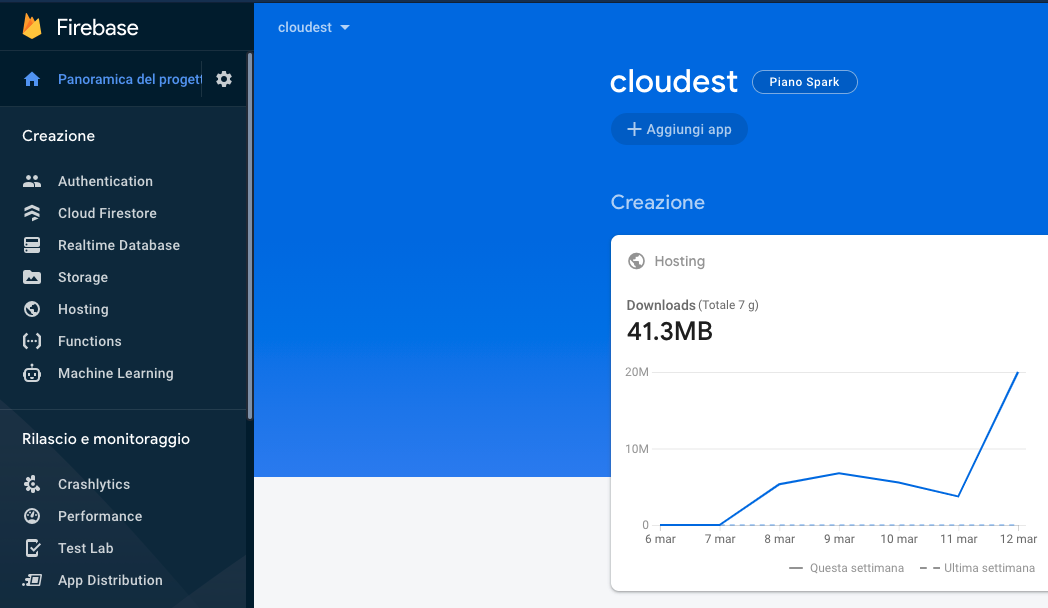
\includegraphics[width=16cm]{images/firebase.png}
  \centering
  \caption{Firebase console}
  \label{fig:firebase}
\end{figure}

\newpage
\addcontentsline{toc}{section}{References}
\begin{thebibliography}{1}

\bibitem{seed_scientific_article} 
SeedScientific Article, \href{https://seedscientific.com/how-much-data-is-created-every-day}{https://seedscientific.com/how-much-data-is-created-every-day},
\textit{How Much Data Is Created Every Day?}, Branka Vuleta, 28 Gen - 2021.

\bibitem{truffle_suite}
Truffle Suite, \href{https://www.trufflesuite.com/}{https://www.trufflesuite.com/}, ConsenSys Software Inc.

\bibitem{solidity}
Solidity Language, \href{https://soliditylang.org/}{https://soliditylang.org/}, Solidity Team

\bibitem{web3js}
Web3JS, \href{https://github.com/ChainSafe/web3.js}{https://github.com/ChainSafe/web3.js}, \textit{Ethereum Javascript API}, ChainSafe

\bibitem{nodejs}
NodeJS, \href{https://nodejs.org/}{https://nodejs.org/}, OpenJS Foundation

\bibitem{reactjs}
ReactJS, \href{https://reactjs.org/}{https://reactjs.org/}, Facebook Inc.

\bibitem{metamask}
Metamask, \href{https://metamask.io/}{https://metamask.io/}, Metamask, a ConsenSys Formation

\bibitem{ganache}
Ganache, \href{https://www.trufflesuite.com/ganache}{https://www.trufflesuite.com/ganache}, ConsenSys Software Inc.

\bibitem{kovan}
Kovan Testnet, \href{https://kovan-testnet.github.io/website/}{https://kovan-testnet.github.io/website/}, Parity Technologies

\bibitem{infura}
Infura, \href{https://infura.io/}{https://infura.io/}, Infura Inc.

\bibitem{ipfs}
IPFS, \href{https://ipfs.io/}{https://ipfs.io/}, Protocol Labs

\bibitem{microsoft_planner}
Microsoft Planner, \href{https://www.microsoft.com/en-ww/microsoft-365/business/task-management-software}{https://www.microsoft.com/}, Microsoft

\bibitem{vs_code}
Visual Studio Code, \href{https://code.visualstudio.com/}{https://code.visualstudio.com/}, Microsoft

\bibitem{firebase}
Firebase, \href{https://firebase.google.com/}{https://firebase.google.com/}, Google Developers, Google


\end{thebibliography}
\end{document}


  

































